\chapter{Discussion}

\section{Annotation Effectiveness}

The results from these experiments indicate that of all the types of annotation methodologies, the query annotations provide the best performance at the lowest cost (i.e the time it took to annotate). Utilising multiple annotations can increase the interpolated precision further towards total recall (and in fact at total recall combining all of the annotations achieves the highest precision overall). It is not surprising to see the tag annotations performing badly in both experiments, since these annotations are unable to encode semantic meaning like text and queries. For instance, images that fall into the topic `Building a Computer': the term `building' can have more than one meaning, a physical structure and the act of assembling an object. The tag annotations did poorly in this topic, where the textual annotations did the best -- these contain semantics which the search engine can exploit when ranking images.  What is surprising (at least when using the description as an input query), is that for some topics assessment annotations perform better. This is most likely do to the fact that the weights of annotated concepts allow the search engine to rank these documents higher. The performance of the textual annotations can perhaps be attributed to spelling and grammatical errors; there is difficulty associated with ensuring these errors are corrected during a pre-processing step in addition to blocking incorrect annotations from being entered in the first place.

In retrospective, the concepts for each query should be chosen manually based on the topics: concepts for some topics are not present, resulting in no images found to be relevant in the retrieval task for these topics. When choosing concepts for use in relevance assessment, there is a large overlap between the titles and the descriptions of the topics and this was seen as good enough. Prior to analysing the results of the relevance assessment annotations, it was thought that they might perform only as well as the images retrieved using tag annotations. Similar to tags, the concepts of the relevance assessments do not contain semantic meaning; however unlike tags, each concept is assigned a weighting of how relevant it is to an image. In ascribing weights, the concepts assigned to images are contextualised; now `building' is highly relevant \textbf{and} `computer' is highly relevant, as opposed to another image that may have an equally high weight for `building' but a high weight for `architecture'. The image with the high `computer' concept will be ranked higher because of the weighting; explaining why relevance assessments outperform the tags even though less images are retrieved. The trade-off in the end is that tagging takes half as long for slightly worse retrieval performance. An assumption that can be made for the relevance assessment annotations then is that if more concepts are added that are relevant to the topics, the retrieval effectiveness can be achieved.

In the case of the query annotations performing the best out of the four annotation methodologies, one would assume that it is simply due to the fact that more images are annotated. The results of the relevance assessments indicate that this is not the case -- the effectiveness of the query methodology can not solely be attributed to the number of images annotated. The relevance assessment annotations perform better (where the input query is taken from the description of the topic) than the query, tags, and in some cases the textual annotations, having the least number of images retrieved. It would seem then that the query annotations are highly suited to the experiments where the input query is composed of very few terms (much like a typical query). It is also possible that, being significantly shorter than the textual annotations, there is less error for spelling and grammatical mistakes. Moreover, the low cost of annotation time further makes the query annotation methodology the most attractive option for annotating a collection of lifelog images for use in text-based image retrieval.

\section{Automatic Image Annotation}

In total, there are 6,657 images that the NTCIR-12 LSAT organisers consider relevant from a collection of 88,125 images (only 7.5\%). If images are annotated from the clustering method of sampling images, only 16,014 images (18\% of the data set) could be annotated. Of that, 1,176 images are considered relevant. This is why the second method of sampling images is so important -- the clusters do not provide a good enough distribution of relevant and non-relevant images to annotate if we just pick at random. A distribution that consists of more relevant images than non-relevant images (i.e relevant to topics) would appear to be more appropriate if one is interested in using annotations for training data. Intuitively it would also seem that topics with a high number of relevant images perform badly due to a low number of training examples; and topics with a low number of relevant images achieve above $0$ precision at high recall because these topics have all of their images manually annotated (remember that a \textit{maximum} of $30$ images are chosen from the known relevant images). This intuition is made visible in Figure \ref{fig:learnt-queries}. The query annotations are used as a demonstration as they are the most interesting of all the learnt annotation methodologies in that they are able to retrieve the highest number of images.

\begin{figure}[h]
    \centering
    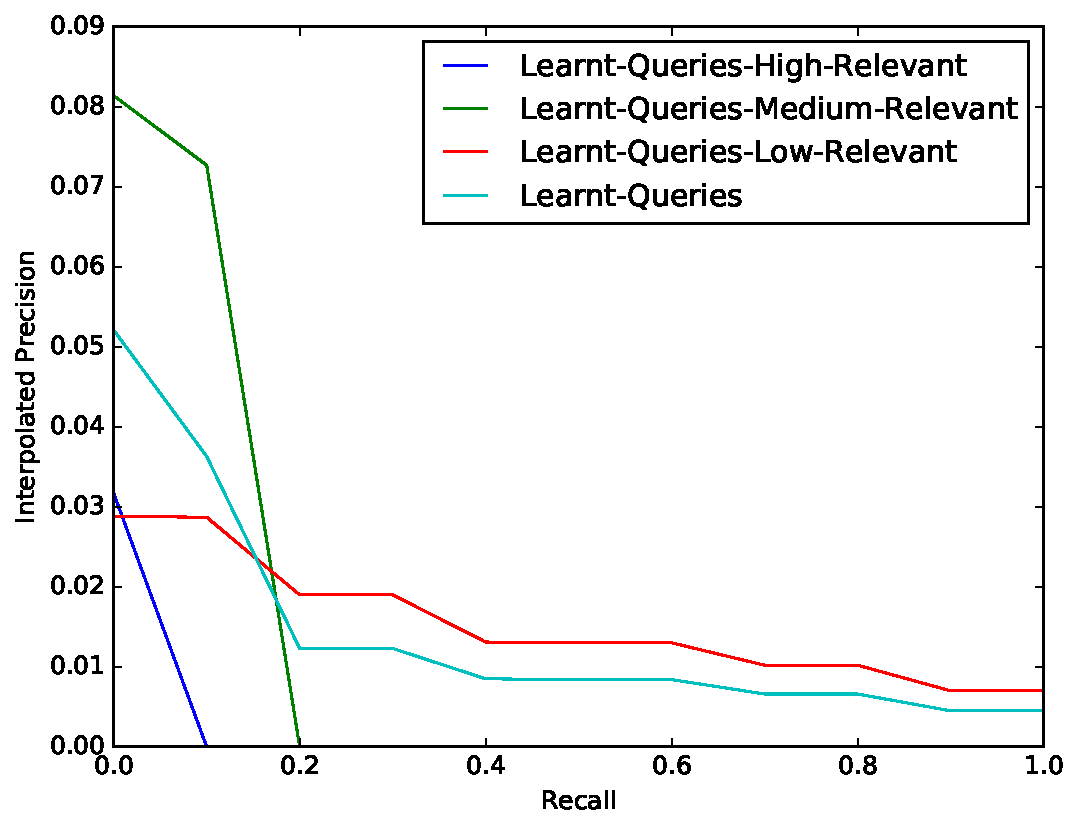
\includegraphics[width=0.95\textwidth]{graphs/learnt-queries}
    \caption{Breakdown of running the same experiment on topics with a large proportion of relevant images (\textgreater 300), the middle number of relevant images (between 100 and 300), and topics with a low number of relevant images (\textless 100)}
    \label{fig:learnt-queries}
\end{figure}

The selection of image to be annotated also intuitively impacts the way a neural network captions images. If a topic contains a diverse range of locations and actions but the images sampled for annotation only cover one of these locations then becomes obvious that many images will get mis-captioned. In hindsight, taking the time to select a variety of perspectives and locations within a moment to cover edge cases could increase the accuracy of the captions; but it is unknown by how much. Another factor that contributes to the poor retrieval effectiveness is the number of training examples required --- there simply may not be enough annotations for the neural network to learn. One thing that can be said for certain is that the number of training iterations required is not the limiting factor in generating accurate captions. Over 200,000 iterations were performed for the three methodologies, and all of them got worse over time. An acceptable number of iterations for this particular setup appears to fall between 30,000 and 100,000; depending on the type of annotation.

The size of the collection and the number of manual annotations is the most likely reason for the poor performance when automatically captioning images. Take for example, the MSCOCO data set~\cite{lin2014microsoft} which contains upwards of 300,000 images with five annotations per image. The number of relevant images in each topic may also be a problem: many topics have a less than 200 relevant images associated with them (around 2\% of the actual collection). The number of images in each topic is detailed in Figure \ref{fig:relevant-images}

\begin{figure}[h]
    \centering
    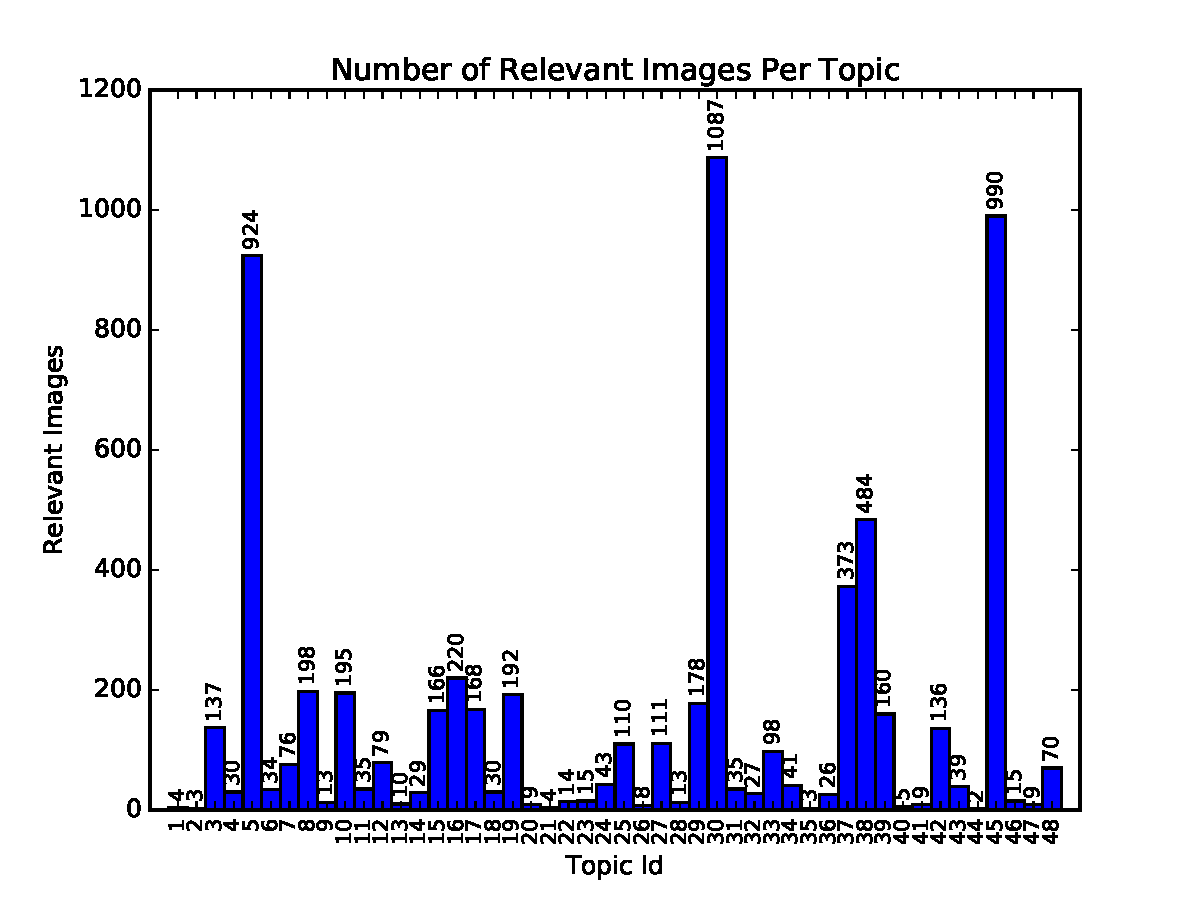
\includegraphics[width=0.95\textwidth]{graphs/relevant-images}
    \caption{Relevant images in each topic}
    \label{fig:relevant-images}
\end{figure}

\section{Interfaces}

The original intent of the topics perhaps does not to imply that images be annotated at random, one-by-one. Relevant images in a topic are actually a group of images, or a `moment'. Each topic has several relevant moments, of which  contain certain images that do not appear to be relevant to the topic at all. As a general rule the images that do not look relevant, even though they were considered to be by the task organisers were not annotated as relevant, are ignored. For instance, in the topic `Conversation while eating', the lifelogger often wipes his mouth with a serviette blocking the camera. These blurry or obscured images are not annotated. Grouping images into moments may also speed up the annotation process: annotating several images considered to be a moment may not only allow collecting annotations less tedious and time consuming, but could also allow for more images to be annotated. The downside to this, however, may be that these irrelevant images crop up inside each moment. One way to avoid a situation like this is to let the annotator remove images that are covered by objects or too blurry to make anything out.

\begin{figure}[h]
    \centering
    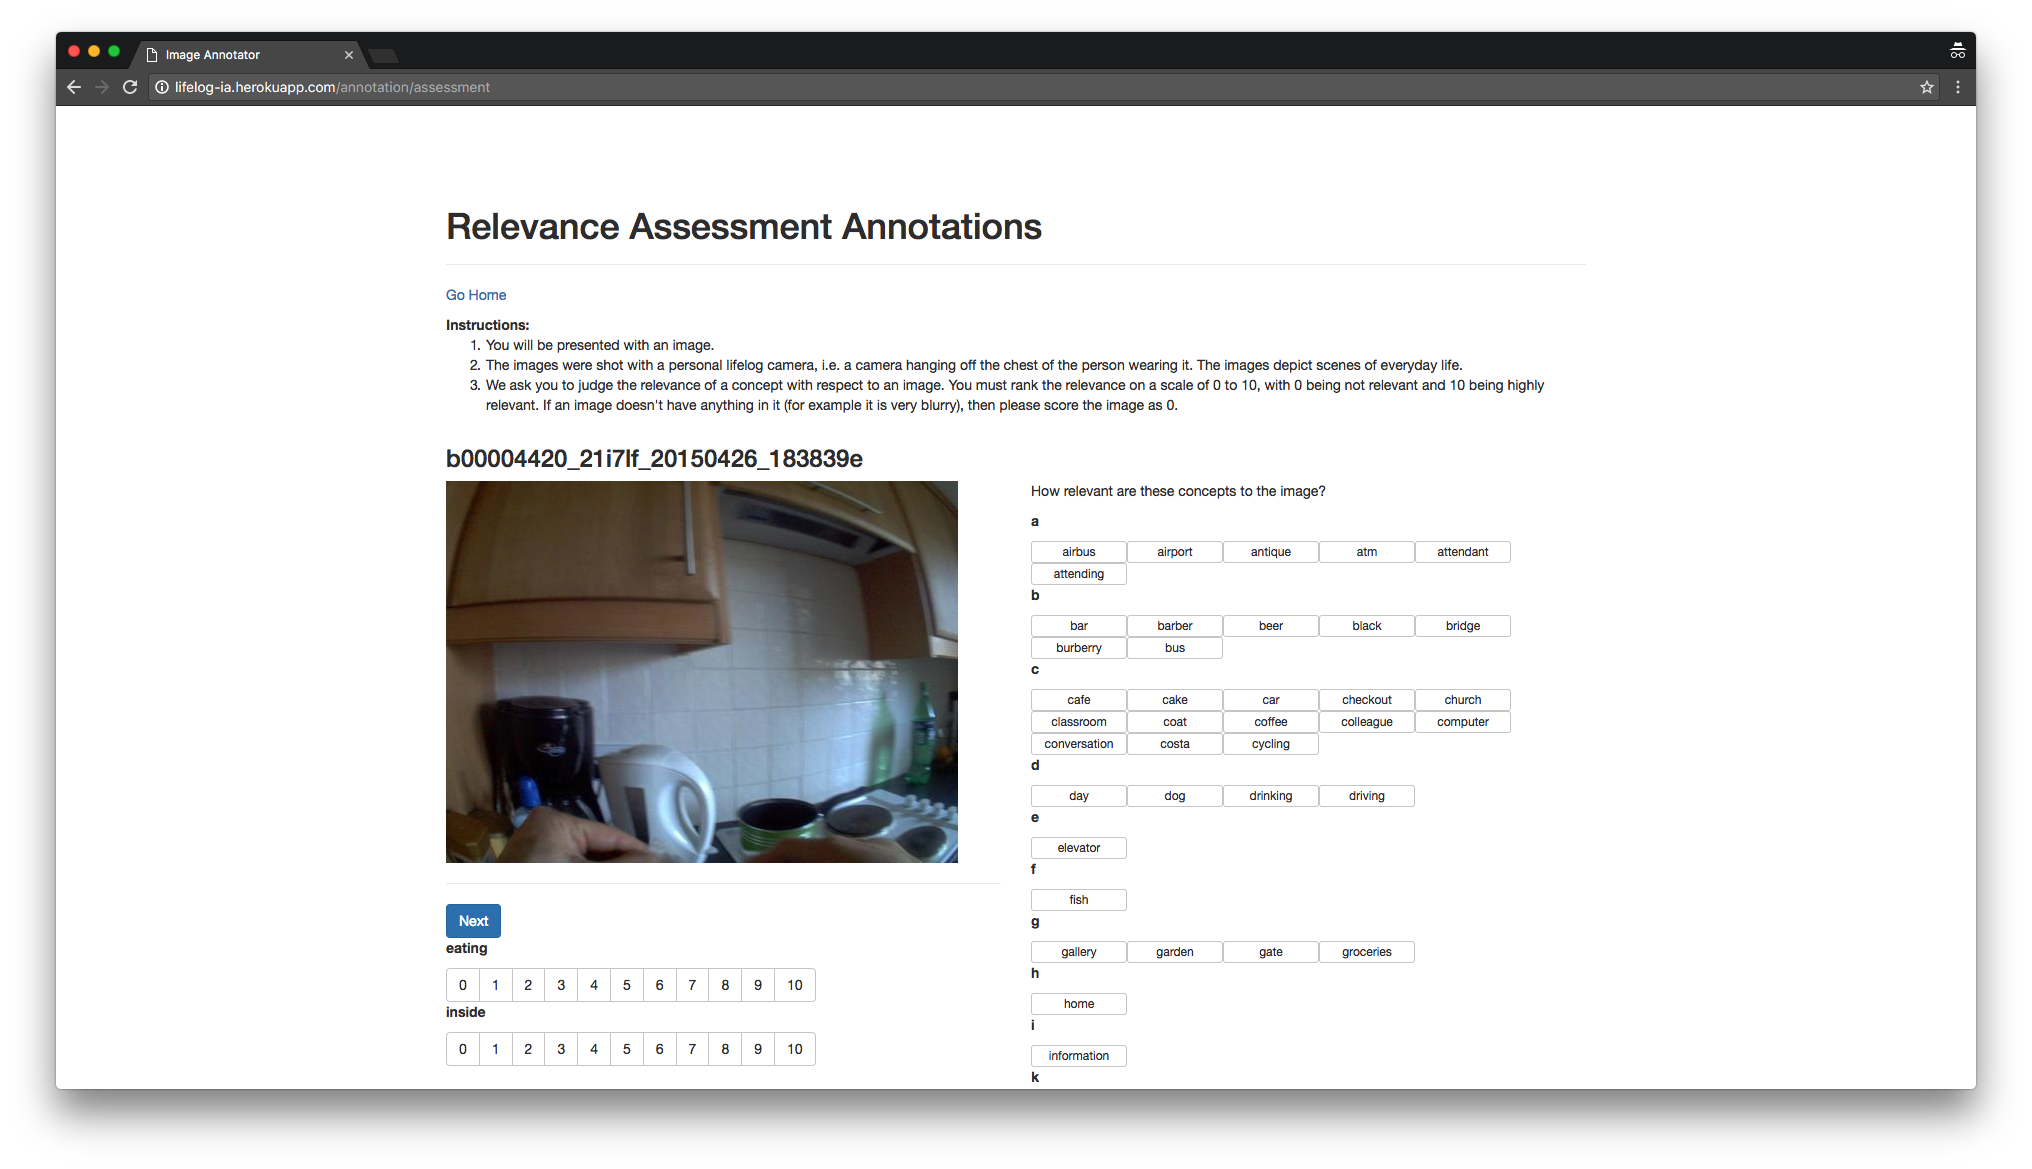
\includegraphics[width=0.95\textwidth]{images/new-rel-ass-interface}
    \caption{Updated query annotation interface}
    \label{fig:new-rel-ass}
\end{figure}

The interfaces themselves are iterative and dynamic while collecting annotations; they change often in response to feedback from annotators. The biggest change from the initial design is the relevance assessment interface, as seen in Figure \ref{fig:new-rel-ass}. Now rather than clicking to judge every concept to the image, each concept is grouped alphabetically; when one is clicked, assessments are added underneath the image. Not every caption must be assessed manually: When the next button is clicked, all unassessed captions are automatically considered not relevant. 




% - While there is an overlap of the terms in the annotations and queries, this does not necessarily mean that the terms in the annotations are used within the same context. This is particularly evident in the tag annotations. The term `key' is relevant to a query where the person wearing a lifelog camera is getting a key replaced, but the term was also found within the context of someone using a `key card' to enter their office.

% The topics were not designed to have images annotated individually out of order. Topics were designed with a range of images that are relevant, or a `moment' of images. 

% - even though images are chosen from random from a smaller pool of images, it simply was not enough to pick at random. The qrels identified 6657 images that should be relevant. From here, the pool of sampled images only contains 1179 images. Only 17.7\% of the images in the images chosen by clustering can be annotated.


% differences between each annotation methodology - All of them are very different to each other, which presents some interesting problems such as how long it takes to annotate each image, how can each annotation methodology be evaluated etc

% text
% Textual annotation are the most time consuming annotation type to collect. Many images contain two or more highly relevant events or `important' objects. Describing these can take annotators up to several minutes each. This is opposed to all the other annotation methodologies where most images can be annotated in a minute or less.

% tags
% In terms of evaluation, tags may be the opposite of textual annotations; intuitively tags should be the best at training an image classifier and are expected to perform the worst when embedded a search task. Tags, however, may be very good at boosting the performance of other annotation types in the search task when combined. For instance, searching on the text \textit{and} tags fields may increase the scores of text annotation alone.

% query
% and therefore it is unknown how well the collected queries will perform in search or for training an image classifier. The level of detail in these annotations will be very low, since most queries should be short in length.
% Much like tags, this annotation type will be very easy to collect. Formulating a query for an image should not takz a significant amount of time. There is the problem of bias \todo{Is there really? I should investigate this further}